\section{Interpretation in simplified models}
The absence of a clear indication for the existence of SUSY in the results of the counting experiment presented in Section~\ref{sec:candcresults} constrains the validity of supersymmetric models. To quantify the impact these results have on the allowed parameter space, they are interpreted in specific signal scenarios. Here, the two simplified models discussed in Section~\ref{sec:models} are examined. 

\subsubsection{Selection efficiencies}
The impact of branching fractions, detector acceptance, and selection efficiencies on the different signal points is shown in Figure~\ref{fig:sigEff} for the example of the central signal region for the fixed-edge (left) and slepton-edge (right) models. Because of the much larger branching fraction into lepton pairs in the case of the slepton-edge model, caused by the presence of the slepton in decay chain, the overall acceptance$\times$efficiency is an order of magnitude larger in this case. As the event kinematics vary depending on the sparticle masses, the efficiency strongly depends on the position of the signal point in the $m_{\sbottom}$-$m_{\secondchi}$ plane. In general, the efficiency is low along the diagonal, where little energy is available for the decay products. Another notable feature is a decrease in efficiency around \secondchi masses of about $\unit{225}{\giga\electronvolt}$ in the case of the slepton-edge model. This is caused by the gaps in the signal acceptance between the three invariant mass regions of the counting experiment. No such effect is visible for the fixed-edge case because the signal is concentrated in the low-mass region in this model.  
\begin{figure}[htbp]
\centering
\begin{minipage}[t]{0.49\textwidth}
  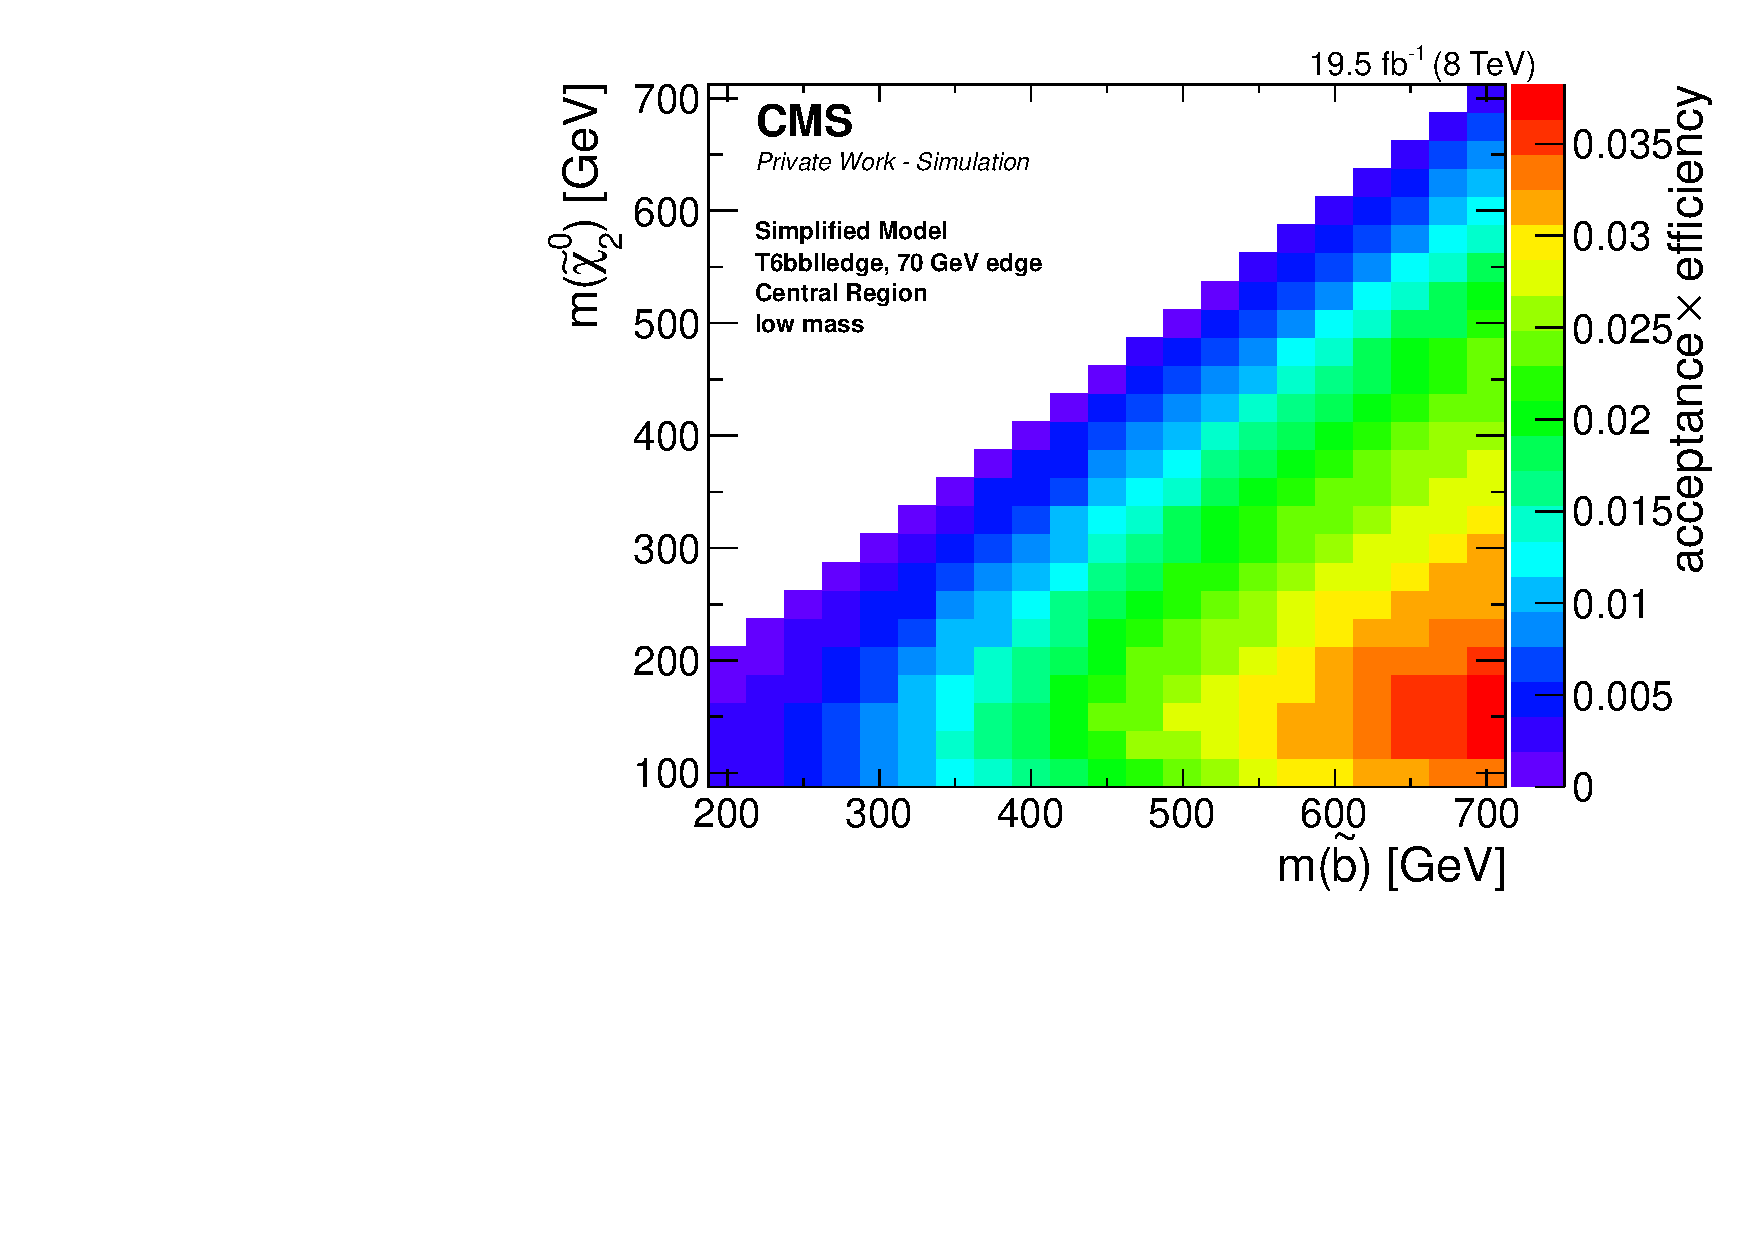
\includegraphics[width=\textwidth]{plots/limits/T6bblledge_70_GeV_Edge_Barrel_lowMll_signalEfficiency.pdf}
\end{minipage}
\begin{minipage}[t]{0.49\textwidth}
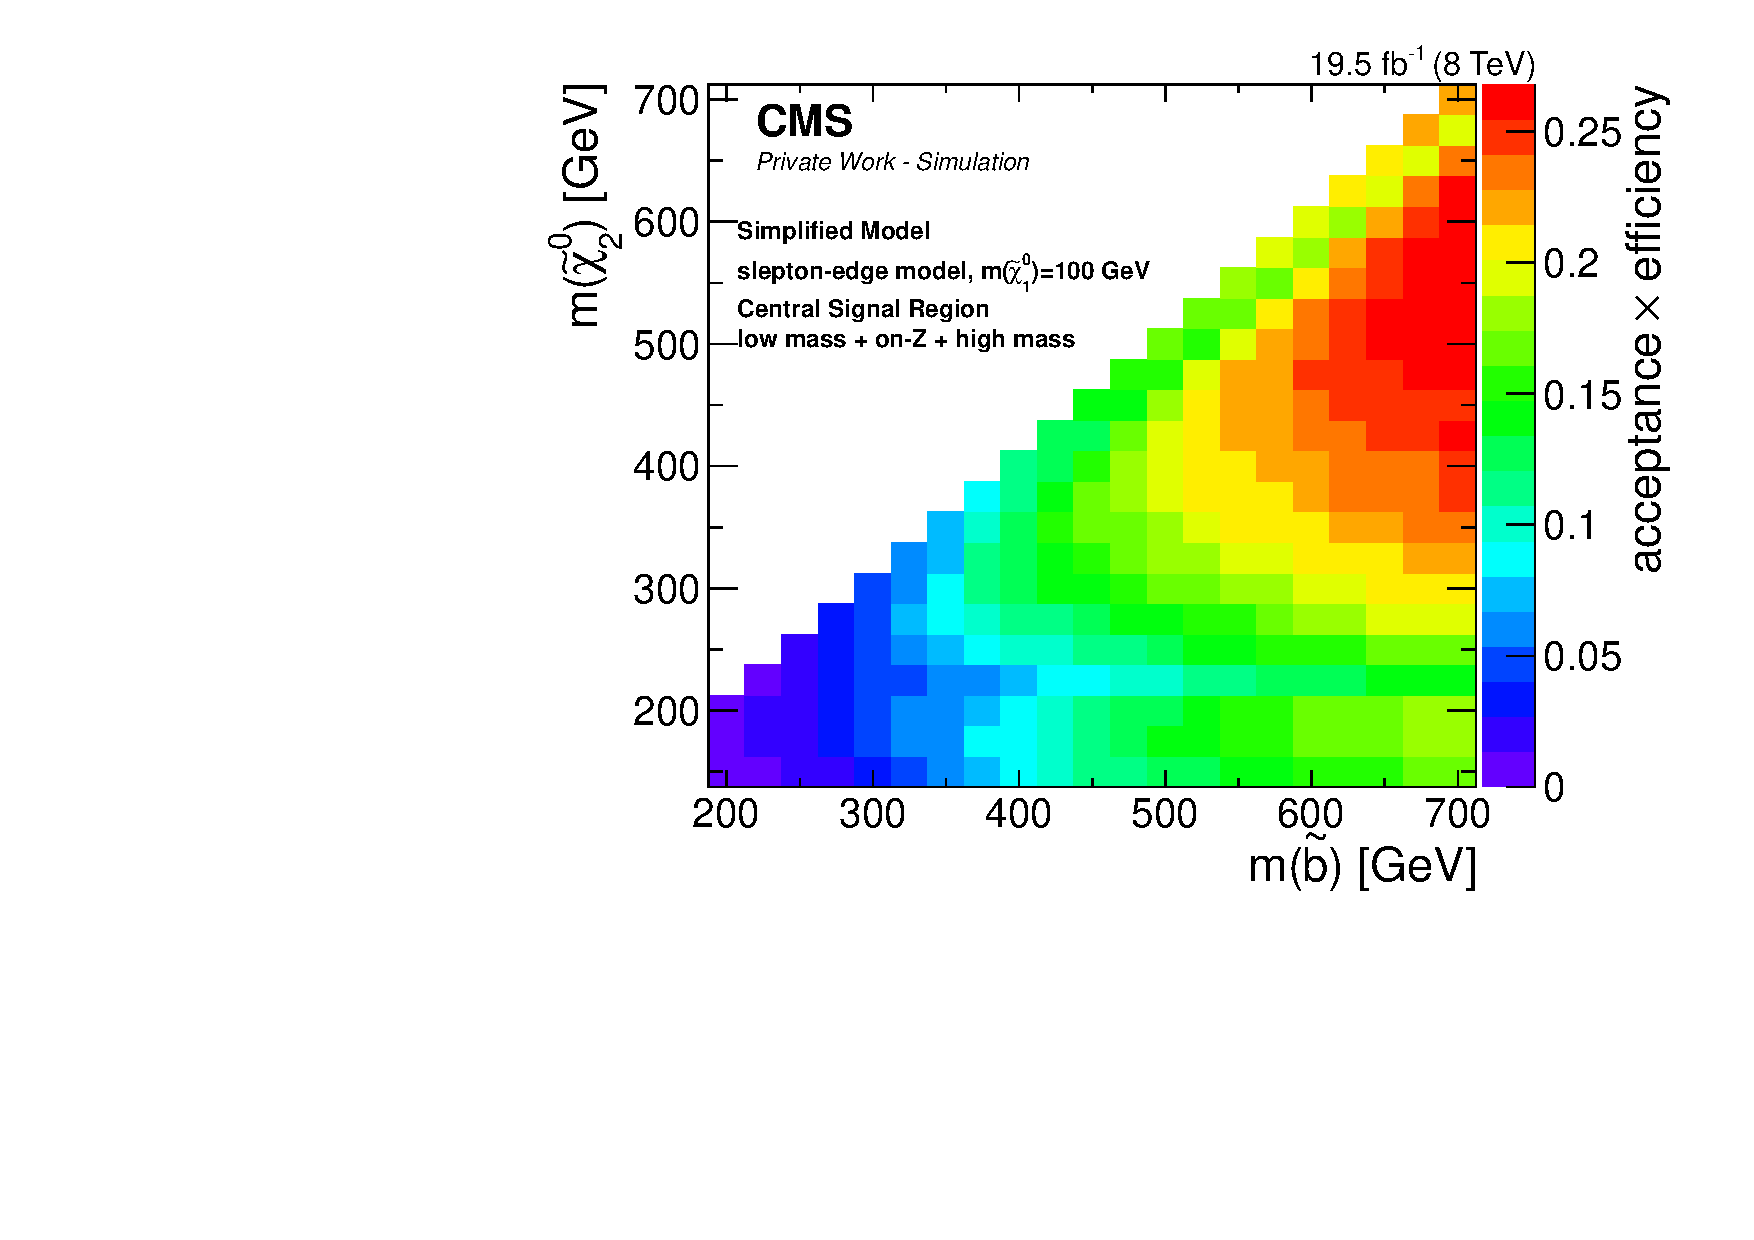
\includegraphics[width=\textwidth]{plots/limits/T6bbllslepton_m_n_1_100_Barrel_signalEfficiency_Reweighted.pdf}
\end{minipage}
\caption{Signal acceptance$\times$efficiency in the $m_{\sbottom}$-$m_{\secondchi}$ plane for the fixed-edge (left) and slepton-edge (right) model for the central signal region.}
\label{fig:sigEff}
\end{figure}
\subsubsection{Systematic uncertainties in signal modelling}
A variety of systematic uncertainties in the signal modelling have to taken into account. The integrated luminosity is measured with a precision of 2.6\%~\cite{CMS-PAS-LUM-13-001}. Variations of the parton distribution functions (PDF) according to the PDF4LHC recommendations~\cite{Alekhin:2011sk,Botje:2011sn,Ball:2012cx,Martin:2009iq,Lai:2010vv} result in an uncertainty of 0--6\% in the signal acceptance. Uncertainties related to lepton efficiencies are of the size of 1\% per lepton. Furthermore, the corrections of the lepton efficiency differences between fast and full detector simulation amount to another 1\% per lepton. The dilepton trigger efficiencies are measured with a precision of 5\%, as described in Section~\ref{sec:triggerEffs}. Uncertainties on the muon momentum scale have negligible impact on the signal acceptance, whereas the uncertainty in the electron energy scale is 0.6\% for central and 1.5\% for forward leptons. Jet energy scale uncertainties~\cite{1748-0221-6-11-P11002} result in an uncertainty in the signal yield of 0--8\%. The uncertainties in the modeling of the objects in the events are propagated to the \MET measurements, resulting in an uncertainty in the signal acceptance of 0--8\%. Here the contributions from the jet energy scale uncertainties are dominant. The events are corrected for a difference between observed data and the modelling of initial-state-radiation (ISR) in Madgraph~\cite{Chatrchyan:2013xna}. Uncertainties in these corrections are propagated to the event selection and result in an uncertainty of 0--14\% in the signal yield.
The uncertainty associated with pileup reweighting is evaluated by shifting the inelastic cross section by $\pm5\%$, resulting in an uncertainty on the signal acceptance of about 1\%. The uncertainties are summarised in Table~\ref{tab:sysUncerts}.

\begin{table}
\begin{center}
\caption{Summary of systematic uncertainties on the signal efficiency.}
\label{tab:sysUncerts}
\begin{tabular}{l|c}
Uncertainty source & Impact on signal yield [\%]\\ \hline 
Luminosity & 2.6 \\
PDFs on acceptance & 0--6 \\ 
Lepton identification/isolation & 2\\
Fast simulation lepton identification/isolation & 2 \\
Dilepton trigger & 5 \\
Lepton energy scale & 0--5  \\
\MET & 0--8  \\
Jet energy scale/resolution & 0--8  \\
ISR modeling & 0--14 \\
Additional interactions & 1 \\
%\multicolumn{2}{c}{Theoretical Uncertainties}\\
%\hline
%Fact./Renorm. Scale and PDFs& 14-18   \\
\end{tabular}
\end{center}
\end{table}
The combined systematic uncertainties are shown in Figure~\ref{fig:sys}. For the most part of the $m_{\sbottom}$-$m_{\secondchi}$ plane the total uncertainty ranges from 5-7\%. However, close to the diagonal the uncertainty increases, caused by a larger impact of JES and ISR uncertainties. This is due to the overall lower jet \pt in this region, increasing the probability for threshold effects around the jet \pt requirement of $\unit{40}{\giga\electronvolt}$. The largest uncertainties are observed for both low masses of the \sbottom and \secondchi, exceeding 20\% for the fixed-edge model and   reaching 15\% for the slepton-edge model.
\begin{figure}[t]
\centering
\begin{minipage}[t]{0.49\textwidth}
  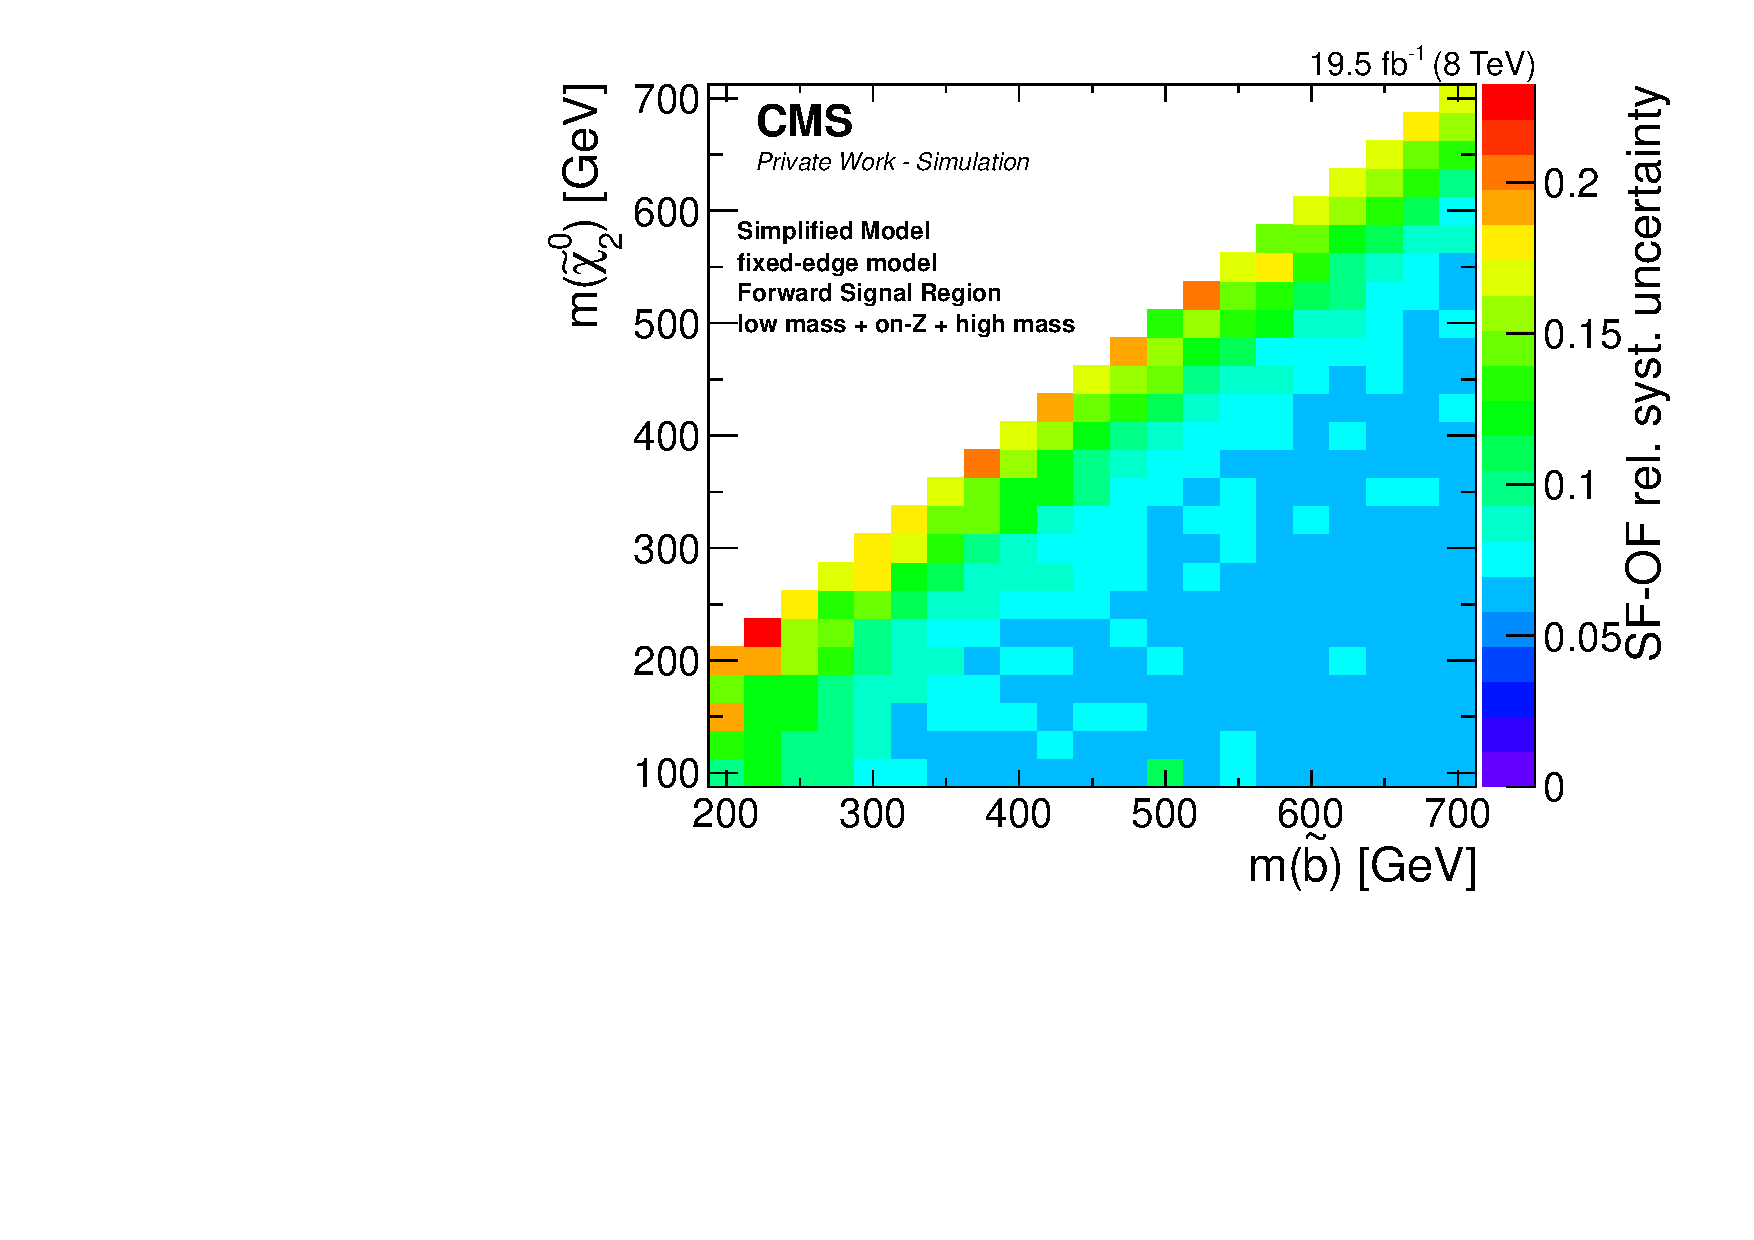
\includegraphics[width=\textwidth]{plots/limits/T6bblledge_70_GeV_Edge_Endcap_syst_err.pdf}
\end{minipage}
\begin{minipage}[t]{0.49\textwidth}
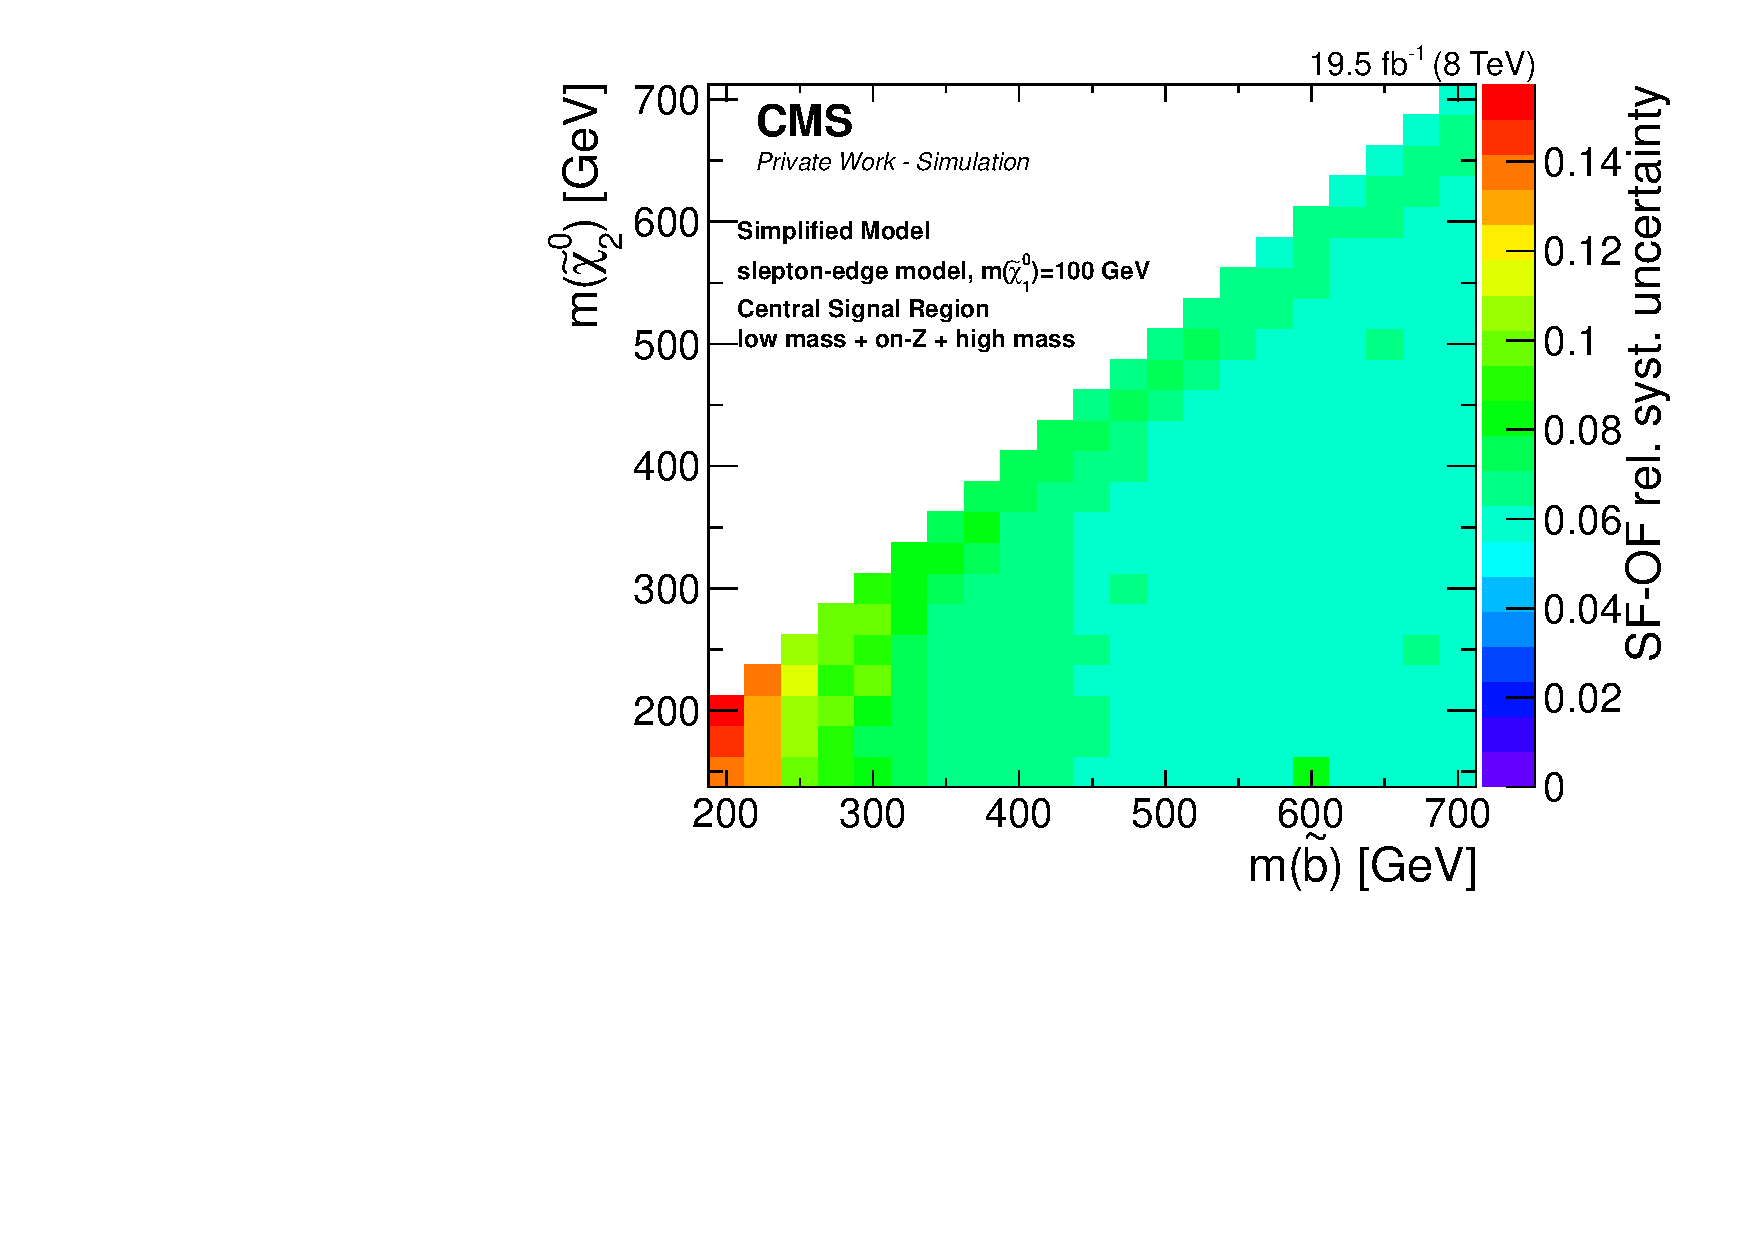
\includegraphics[width=\textwidth]{plots/limits/T6bbllslepton_m_n_1_100_Barrel_syst_err_Reweighted.pdf}
\end{minipage}
\caption{Systematic uncertainty on the signal yield in the central signal region in the $m_{\sbottom}$-$m_{\secondchi}$ plane for the fixed-edge (left) and slepton-edge (right) model.}
\label{fig:sys}
\end{figure}
\subsection{Statistical interpretation}
The results of the counting experiment are translated into exclusion limits by testing the compatibility of the signal plus background ($s+b$) and background only ($b$) hypotheses, treating each signal point in the parameter scans separately. For this purpose, a likelihood function is defined~\cite{HiggsTool1}
\begin{equation}
\label{eq:like}
\mathcal{L}(\text{data}|\mu,\theta) = \text{Poisson}\left(data|\mu\cdot s\left(\theta\right) + b\left(\theta\right)\right)\cdot p\left(\tilde{\theta}|\theta\right),
\end{equation}
where $\mu$ is the signal strength parameter, $\mu = 0$ corresponding to the background only hypothesis and $\mu > 0$ to the  $s+b$ hypothesis, and $p(\tilde{\theta}|\theta)$ parametrises the nuisance parameters $\theta$, with $\tilde{\theta}$ being the nominal value of these parameters. Based on these likelihoods, a test statistic is defined utilizing a profile likelihood ratio: 
\begin{equation*}
\tilde{q_{\mu}} = -2 \ln\frac{\mathcal{L}\left(\text{data}|\mu,\hat{\theta}_\mu\right)}{\mathcal{L}\left(\text{data}|\hat{\mu},\hat{\theta}\right)},
\end{equation*}
where the $\hat{\theta}_\mu$ represent the maximum likelihood estimators for the nuisance parameters for a given $\mu$, whereas $\hat{\mu}$ and $\hat{\theta}$ indicate the global maximum of the likelihood. For the parametrisation of the nuisance parameters $p\left(\tilde{\theta}|\theta\right)$ in Equation~\ref{eq:like}, log-normal distributions are chosen. The distribution of the test statistics is then sampled dicing pseudo-experiments for $\mu > 0$ and $\mu = 0$, representing the $s+b$ and $b$ hypotheses that are tested. The p-values $p_{s+b}$ and $p_{b}$ are defined as the probability to obtain a value of the test statistics as large or larger than the one observed in data for the given hypothesis. To obtain the upper limit on the signal cross section the value of $\mu$ is chosen where $\mathrm{CL}_{\mathrm{s}} = \frac{p_{s+b}}{p_b}$ equals 0.05, corresponding to a 95\% confidence level (CL). In the calculation, all six bins of the counting experiment are combined by multiplying the likelihoods of the different channels. In this procedure, all uncertainties on both background and signal are assumed to be uncorrelated among each other but fully correlated among the different bins. Considered are all uncertainties summarized in Table~\ref{tab:sysUncerts} for the signal and in Table~\ref{tab:METresults2012} for the background.

The resulting exclusion limits are shown in Figure~\ref{fig:limits}. The left plot shows the exclusion limit in the $m_{\sbottom}$-$m_{\secondchi}$ plane for the fixed-edge model. As this model is specifically tuned to provide signals consistent with the excess observed in the low-mass central signal region, the observed limit on $m_{\sbottom}$ deviates from the expected one by about $\unit{75}{\giga\electronvolt}$. Within the assumption of this model, \sbottom masses up to about $\unit{375}{\giga\electronvolt}$ are excluded, depending on the mass of the \secondchi. The right plot shows the limit for the slepton-edge model. Because of the much larger branching fraction into leptons in this model, higher masses can be excluded. The expected limit reaches \sbottom masses of about $\unit{600}{\giga\electronvolt}$ roughly independent of $m_{\secondchi}$, except for the region around $m_{\secondchi} = \unit{225}{\giga\electronvolt}$, where it drops below $\unit{550}{\giga\electronvolt}$, because of the gaps in acceptance discussed above. For lower $m_{\secondchi}$ the observed limit is significantly weaker than the expected, as here the limit is dominated by the low-mass signal region in which the excess was observed. For higher $m_{\secondchi}$, the observed limit agrees with the expected within one standard deviation. The observed lower limit on $m_{\sbottom}$ ranges from $\unit{470}{\giga\electronvolt}$ to $\unit{590}{\giga\electronvolt}$, depending on $m_{\secondchi}$.
\begin{figure}[htbp]
\centering
\begin{minipage}[t]{0.49\textwidth}
  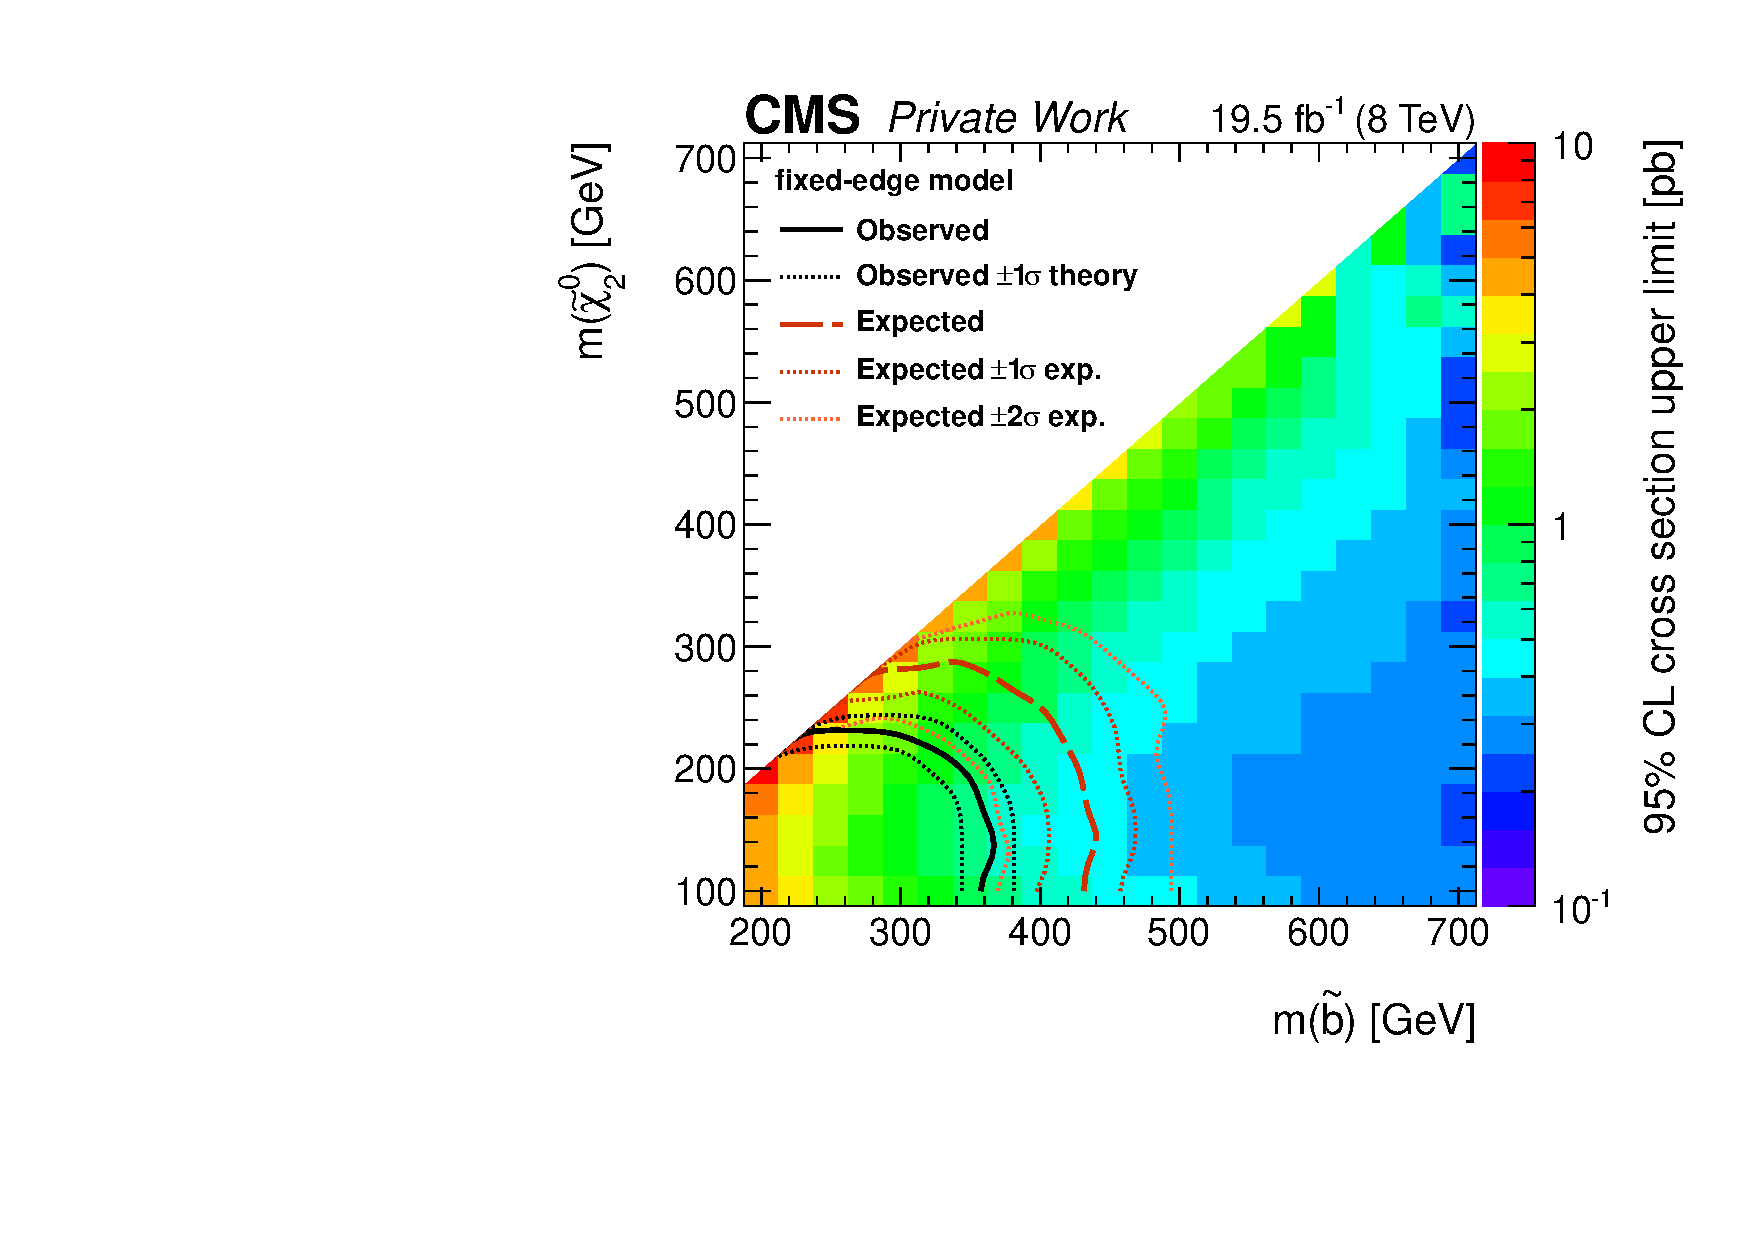
\includegraphics[width=\textwidth]{plots/limits/Fixed_Edge_sbottom_neutralino2_Exclusion_witXsecLimit.pdf}
\end{minipage}
\begin{minipage}[t]{0.49\textwidth}
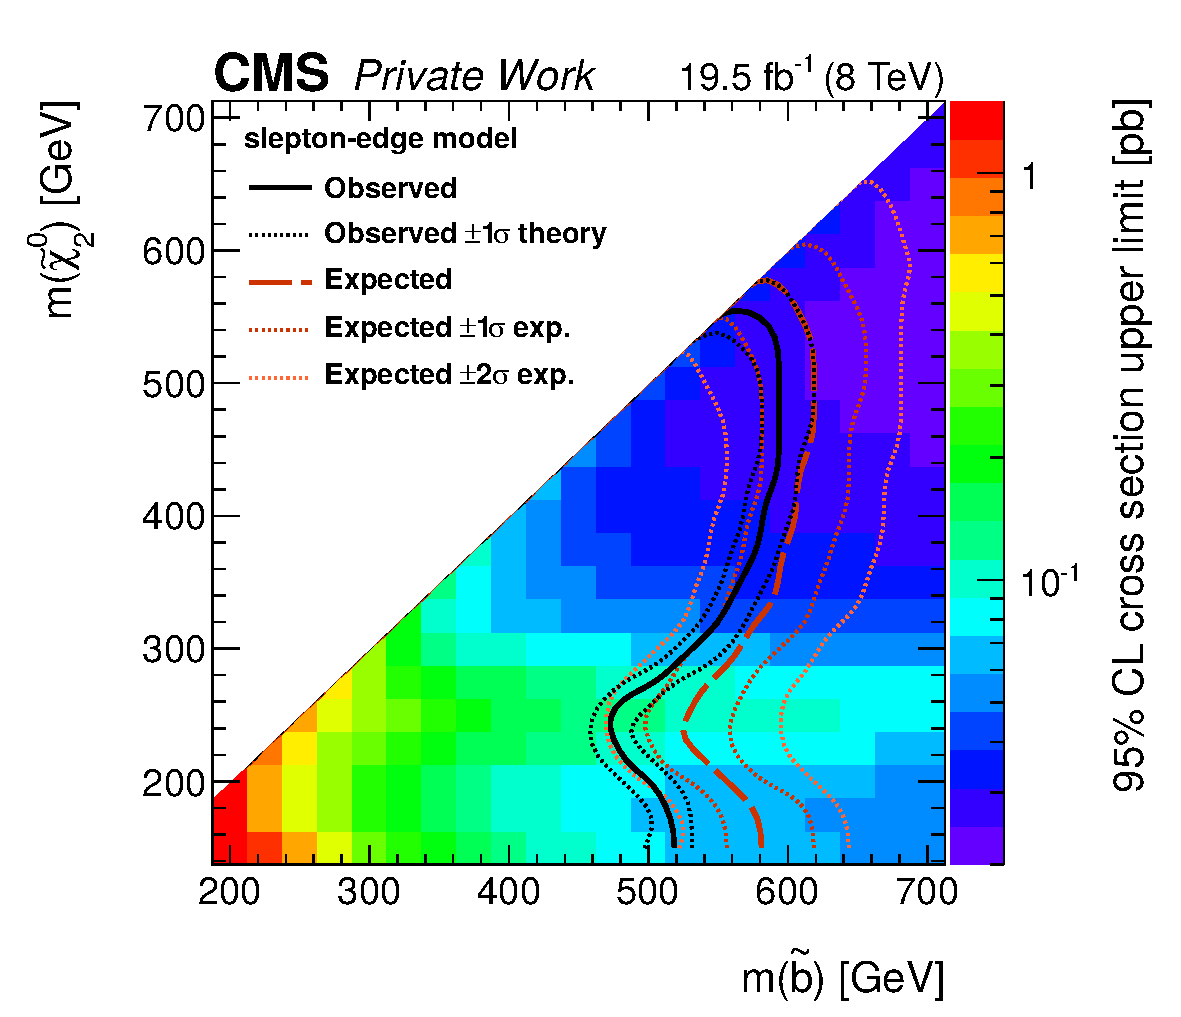
\includegraphics[width=\textwidth]{plots/limits/Fixed_Neutralino_sbottom_neutralino2_Exclusion_witXsecLimit.pdf}
\end{minipage}
\caption{Exclusion limits in the $m_{\sbottom}$-$m_{\secondchi}$ plane for the fixed-edge (left) and slepton-edge (right) model. For each signal point the upper cross section limit is shown colour coded. The intersection of the theoretical cross section with the cross section limit is shown as a solid black line, with every signal point to the left and below the curve being excluded. The $1-\sigma$ theoretical uncertainty interval on the observed limit is shown as dotted black lines. The expected limit together with the $1-$ and $2-\sigma$ experimental uncertainty intervals are shown as brownish solid and dashed lines.}
\label{fig:limits}
\end{figure}